\documentclass[tikz]{standalone}

\usetikzlibrary{positioning}

\begin{document}
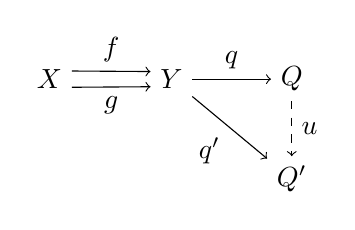
\begin{tikzpicture}
	\node (X) {$X$};
	\node [right=1.0cm of X] (Y) {$Y$};
	\node [right=1.0cm of Y] (Q) {$Q$};
	\node [below=0.7cm of Q] (Q') {$Q'$};
	\draw [->] (X.20) to node [above] {$f$} (Y.160);
	\draw [->] (X.340) to node [below] {$g$} (Y.200);
	\draw [->] (Y) to node [above] {$q$} (Q);
	\draw [->, dashed] (Q) to node [right] {$u$} (Q');
	\draw [->] (Y) to node [below left] {$q'$} (Q');
\end{tikzpicture}
\end{document}
